\setcounter{section}{69}
\section{Дерево Фенвика: классическая задача, операции update и getSum. }
\textbf{Дерево Фенвика} (англ. Binary indexed tree) — структура данных, требующая $O(n)$ памяти и позволяющая эффективно (за $O(\log n)$) выполнять следующие операции:
\begin{itemize}
    \item изменять значение любого элемента в массиве,
    \item выполнять некоторую ассоциативную, коммутативную, обратимую операцию $\circ$ на отрезке $[i,j]$.
\end{itemize}
\par \noindent Пусть дан массив $a_1, \ldots, a_{n-1}$ и задача найти сумму на отрезке $[l,r]$.
\newline Тогда \textbf{деревом Фенвика} будем называть массив $T$ из $n$ элементов: $T_i=\sum_{k=F(i)}^{i}a_k$, где $i=0\ldots n-1$ и $F(i)$ — некоторая функция, от выбора которой зависит время работы операций над деревом.
Введём две функции $F(x)=x \; \& \; (x+1)$ и $G(x)=x \; | \; (x+1)$. \newline Заметим, что для этих функций верно: $F(x)\leq x; \quad G(x) \geq x+1$
\\ \par \textbf{Запрос суммы:} Когда нам нужна сумма на отрезке, мы будем сводить этот запрос к двум суммам на префиксе: $sum(l,r)=pref(r)-pref(l-1)$. Оба этих запроса будем считать по формуле $pref(i) = T_i+pref(F(i)-1)$
\begin{figure}[h]
\centering
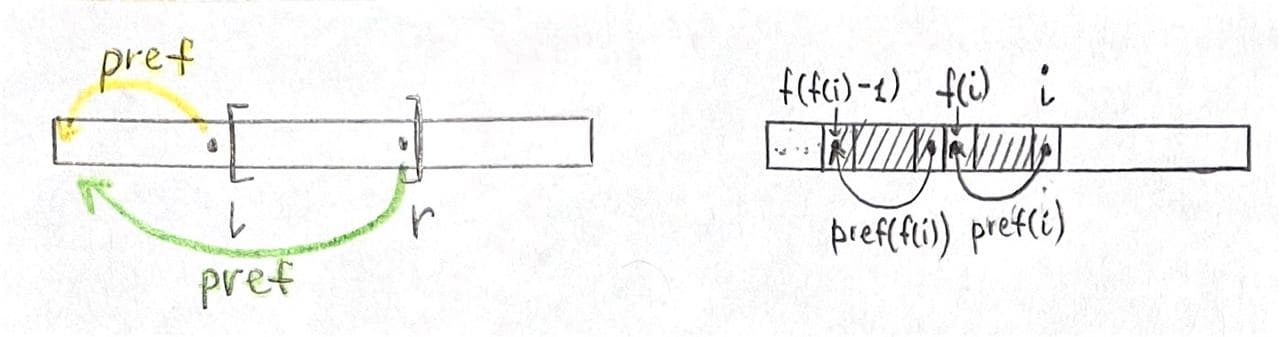
\includegraphics[width=1\linewidth]{images/70-75_fenwick}
\end{figure}
\par \textbf{Оценим время работы запроса суммы:}
\newline \begin{minipage}{0.3\textwidth}
  \begin{flushleft}
	$$
    \begin{array}{r}
    \begin{array}{r}
    i \;| \ldots01111\\
    \end{array} \\
    \hline
    \begin{array}{r}
    i+1 \;| \ldots10000\\
    F(i) \;| \ldots00000\\
    \end{array} \\
    \hline
    \begin{array}{r}
    F(i)-1 \;| \ldots11111\\
    \end{array}
    \end{array}
    $$
  \end{flushleft}
\end{minipage}
\begin{minipage}{0.7\textwidth}
\vspace{2ex}
  \begin{flushright}
	$F(i)$ зануляет последний блок из единиц. \newline При переходе $i \mapsto F(i)-1$ младший 0 превращается в 1 и где-то в начале числа появляется 0.
	\newline В числе $n$ имеется $\log_{2}{n}$ бит. Следовательно, время работы $\leq \log_{2}{n} \; \Rightarrow \; O(\log n)$
  \end{flushright}
\end{minipage}
\\ \\ \par \textbf{Запрос обновления:} Когда мы изменяем 
$k$-ю ячейку исходного массива, мы обновляем все $T_i$, в которых учтена эта ячейка.
\\ \par \textbf{Оценим время работы запроса обновления:}
\newline \begin{minipage}{0.3\textwidth}
  \begin{flushleft}
	$$
    \begin{array}{r}
    \begin{array}{r}
    i \;| \ldots11111\\
    pos \;| \ldots0 \cdot \cdot \cdot\cdot \\
    F(i) \;| \ldots00000\\
    \end{array} \\
    \hline
    \begin{array}{r}
    i\text{*} \;| \ldots01011\\
    F(i\text{*}) \;| \ldots01000\\
    \end{array} \\
    \end{array}
    $$
  \end{flushleft}
\end{minipage}
\begin{minipage}{0.7\textwidth}
\vspace{2ex}
  \begin{flushright}
    Найдем все такие $i$, что $F(i) \leq pos \leq i$, что бы сделать $T_i =T_i + val$
	\newline Заметим, что при рассмотрении какого-то 0 в $pos$, мы берем $i$, в котором на всех следующих позициях 1, иначе возникает противоречие с $F(i) \leq pos$ (случай с *)
	\newline При переходе $i \mapsto G(i)$ младшиий 0 превращается в 1.
	\newline В числе $n$ имеется $\log_{2}{n}$ бит. Следовательно, время работы $\leq \log_{2}{n} \; \Rightarrow \; O(\log n)$
  \end{flushright}
\end{minipage}
Например, если $pos=01001$, то $i = 01001, \; 01011, \; 01111, \; 11111$
\par \textbf{Построение:} 
\begin{itemize}
    \item 1 способ за $O(n)$: Построить массив префиксных сумм $p_0=a_0 \;\; p_{i+1}=a_{i+1}+p_i$ и тогда $T_i = p_i - p_{F(i)-1}$.
    \item 2 способ за $O(n\log n)$: Построить пустой $T$ и сделать $n$ обновлений.
\end{itemize}
\lstinputlisting[language=C++,
emph={int,char,double,float,unsigned},
emphstyle={\color{blue}}
]{code/70-75_main.cpp}

\newpage
\setcounter{section}{70}
\section{Обобщение дерева Фенвика на большие размерности. Изменение асимптотики. }

\textbf{Многомерное дерево Фенвика} (англ. Multidimensional Binary Indexed Tree) — структура данных, требующая $O(n^k)$ памяти и позволяющая эффективно (за $O(\log^k n)$)
изменять значение любого элемента в k-мерном массиве;
выполнять некоторую ассоциативную, коммутативную, обратимую операцию $\circ$ на $k$-мерном прямоугольнике $[i_1,\ldots,i_k]$;
где $n$ - максимальное значение для каждой координаты.
\\ \par \noindent Рассмотрим для начала дерево Фенвика на примере $k$-мерного массива с $k=2$, а затем посмотрим, как можно обобщить его на большие размерности.
\newline Пусть дан массив $A$ из $n\times m$ элементов: $a_{i,j}$.
\textbf{Деревом Фенвика} будем называть массив $T$ из $n\times m$ элементов: $$T_{i,j}=\sum_{k=F(i)}^{i}\sum_{q=F(j)}^{j}a_{k,q}$$ где $F(i)=i \; \& \; (i+1)$, как и в одномерном дереве Фенвика.
\\ \par \textbf{Пример задачи для двумерного случая}
\par \noindent Пусть имеем набор точек на плоскости с неотрицательными координатами. Определены 3 операции:
\begin{enumerate}
    \item добавить точку в $(x,y)$;
    \item удалить точку из $(x,y)$;
    \item посчитать количество точек в прямоугольнике $(0,0),(x,y)$;
\end{enumerate}
Пусть $n$ — количество точек, $\max X$ — максимальная $X$ координата, $\max Y$ — максимальная $Y$ координата.
Тогда дерево строится за $O(n\cdot \log (\max X)\cdot \log (\max Y))$, а запросы выполняются за $O(\log (\max X)\cdot \log (\max Y))$

Добавляя точку вызовем $update(x,y,1)$, а удаляя $update(x,y,-1)$. Таким образом запрос $sum(x,y)$ дает количество точек в прямоугольнике. \newline

\begin{wrapfigure}{R}{0.4\textwidth}
\vspace{-6ex}
\centering
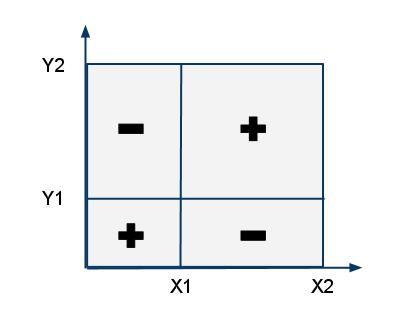
\includegraphics[width=0.4\textwidth]{images/70-75_vvk}
\end{wrapfigure}


\par \textbf{Замечание: } В коде добавляется лишь двухуровневая вложенность циклов.
\\ \par \noindent Чтобы посчитать значение функции для прямоугольника $(x_1,y_1),(x_2,y_2)$ нужно воспользоваться \textbf{формулой включения-исключения}. Например, для суммы: $s=sum(x_2,y_2)-sum(x_2,y_1-1)-sum(x_1-1,y_2)+sum(x_1-1,y_1-1)$
\newline \newline \par \textbf{Обобщение на большие размерности}
 \par \noindent  Дерево Фенвика относится к структурам данных, требующим малое количество дополнительной памяти. В комбинации с простым представлением тривиального случая данной структуры это дает возможность легко повышать размерность дерева Фенвика, в котором в ячейках какого-то фиксированного уровня будет находиться дерево меньшей размерности. Для его реализации нам достаточно во всех операциях для каждой новой размерности просто добавить вложенный цикл, пробегающий в ней соответствующие индексы.


\newpage
\setcounter{section}{71}
\section{Обратное (встречное) дерево Фенвика: максимум на отрезке и изменение (увеличение) в точке. }
\textbf{Встречное дерево Фенвика} (англ. counter tree Fenwick) — дерево Фенвика, в котором над каждым столбцом идет столбец такой же высоты.

\begin{figure}
\begin{minipage}[h]{0.47\linewidth}
\center{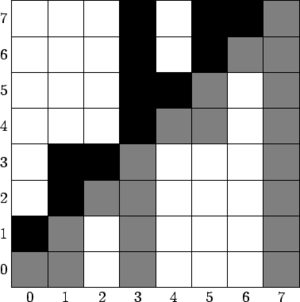
\includegraphics[width=0.85\linewidth]{images/70-75_2tree}} Встречное дерево Фенвика \\
\end{minipage}
\hfill
\begin{minipage}[h]{0.47\linewidth}
\center{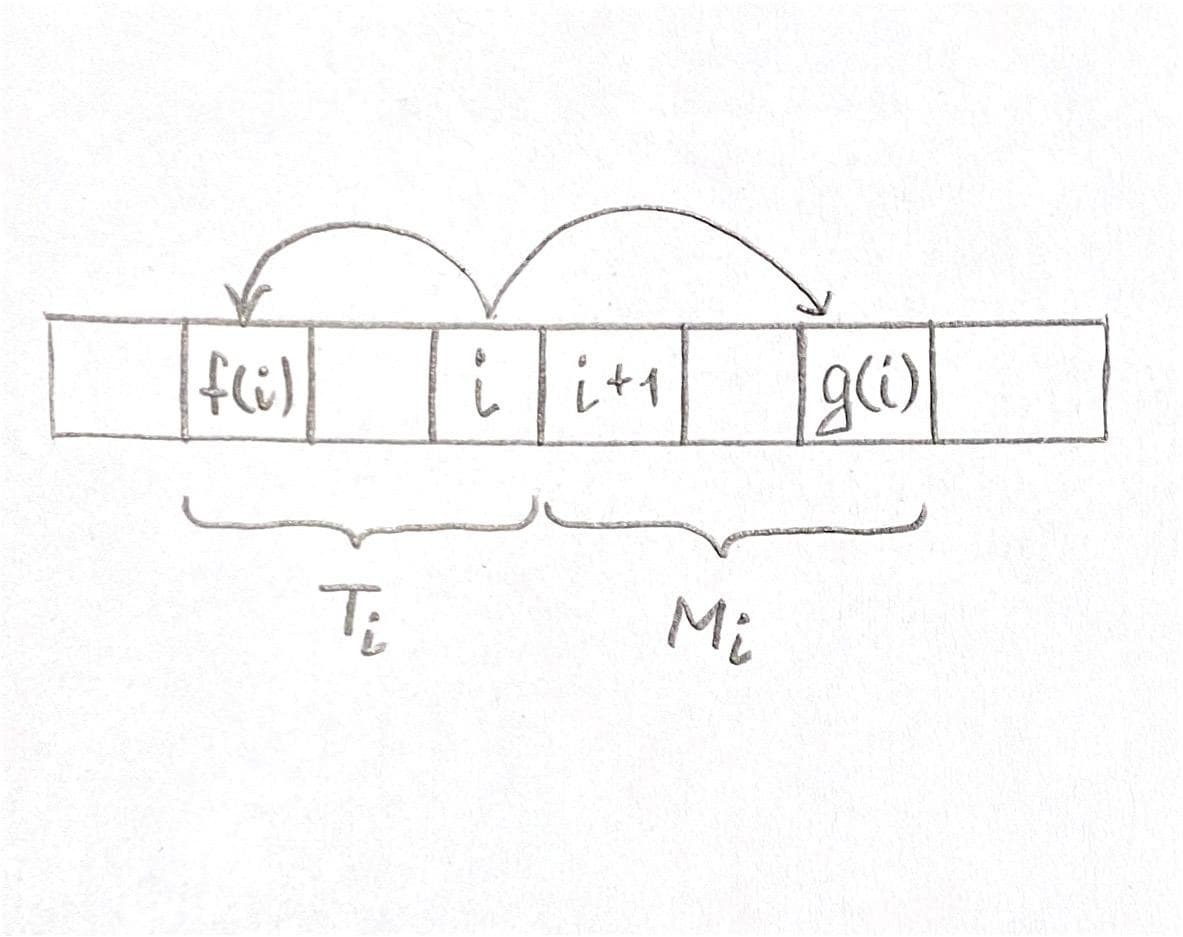
\includegraphics[width=1\linewidth]{images/70-75_111}} \\Покрытие элемента $a_i$
\end{minipage}
\end{figure}
Таким образом встречное дерево Фенвика хранит два массива:
$$T_i=\sum_{k=F(i)}^{i}a_k \qquad M_i =\sum_{k=i+1}^{G(i)}a_k$$
\par \textbf{Запрос обновления:} Когда мы изменяем 
$k$-ю ячейку исходного массива, мы обновляем все $T_i$ и $M_i$, в которых учтена эта ячейка.
\\ \par \textbf{Оценим время работы запроса обновления:}
\newline \begin{minipage}{0.3\textwidth}
  \begin{flushleft}
	$$
    \begin{array}{r}
    \begin{array}{r}
    i \;| \ldots01111\\
    i+1 \;| \ldots10000\\
    pos \;| \ldots1 \cdot \cdot \cdot\cdot \\
    G(i) \;| \ldots11111\\
    \end{array} \\
    \hline
    \begin{array}{r}
    (i+1)\text{*} \;| \ldots10010\\
    G((i+1)\text{*}) \;| \ldots10011\\
    \end{array} \\
    \end{array}
    $$
  \end{flushleft}
\end{minipage}
\begin{minipage}{0.7\textwidth}
\vspace{2ex}
  \begin{flushright}
    Найдем все такие $i$, что $i+1 \leq pos \leq G(i)$, что бы сделать $M_i=M_i + val$
	\newline Заметим, что при рассмотрении какой-то 1 в $pos$, мы берем $i+1$, в котором на всех следующих позициях 0, иначе возникает противоречие с $G(i) \geq pos$ (случай с *)
	\newline В числе $n$ имеется $\log_{2}{n}$ бит. Поэтому, время обновления  $T_i \text{ и } M_i \quad \leq 2\log_{2}{n} \; \Rightarrow \; O(\log n)$
  \end{flushright}
\end{minipage}
\\ \par \textbf{Запрос суммы:} Здесь и происходит вся магия позволяющая нам использовать необратимые операции. Необходимо найти сумму на $(l;r]$, то есть $sum(l,r)=\sum_{i=l+1}^{r}a_i$.
\lstinputlisting[language=C++,
emph={int,char,double,float,unsigned},
emphstyle={\color{blue}}
]{code/70-75_code.cpp}
Таким образом, мы прыгаем по отрезку от правого конца $r$ до тех пор, пока $F(r)$ лежит в отрезке. Затем прыгаем от $l$ до тех пор, пока $G(l)$ лежит в отрезке. Заметим, что $l'$ и $r'$ всретятся в некоторой ячейке, так как из $F(r) \leq l$ и $r > l$ следует, что $G(l) \leq r$
\newline \begin{minipage}{0.3\textwidth}
  \begin{flushleft}
	$$
    \begin{array}{r}
    \begin{array}{r}
    r \;| \ldots11111\\
    l \;| \ldots0\cdot \cdot \cdot \cdot\\
    F(r) \;| \ldots00000\\
    \end{array} \\
    \hline
    \begin{array}{r}
    r\text{*} \;| \ldots11011\\
    F(r\text{*}) \;| \ldots11000\\
    \end{array} \\
    \hline
    \begin{array}{r}
    l_1 \;| \ldots01011\\
    G(l_1) \;| \ldots01111\\
    l_2 \;| \ldots01111\\
    G(l_2) \;| \ldots11111\\
    \end{array}
    \end{array}
    $$
  \end{flushleft}
\end{minipage}
\begin{minipage}{0.7\textwidth}
\vspace{2ex}
  \begin{flushright}
	Для начала заметим, что в весь хвост $r$ равен 1, так как иначе реализуется случай с $r\text{*}$ и выходит противоречие с условием $F(r) \leq l$. Далее, из прелставленной конфигурации следует, что $G(l) \leq r$. При этом на последнем шаге (как в случае $l_2$) мы получаем равенство $G(l)=r$ из чего следует, что отрезок схлопнется.
  \end{flushright}
\end{minipage}
\par \textbf{Замечание:} Данная структура данных легко обобщается на случай многомерных массивов.
\\ \par \noindent При поиске максимума на отрезке нужно учесть тот факт, что мы не можем уменьшать значение в массиве, так как иначе максимум будет возможно определён не корректно, поэтому при update: $a_{pos} = \max \{a_{pos},val\}$

\setcounter{section}{72}
\section{Дерево Фенвика: отложенные операции увеличения и запрос суммы на отрезке}

\par \noindent Пусть дан массив $a_1, \ldots, a_{n-1}$ и возможны запросы двух видов:
\begin{enumerate}
    \item найти сумму на отрезке $[l,r]$
    \item увеличить все элементы на отрезке $[l,r]$ на $val$
\end{enumerate}
Рассмотрим массив $B_i$ разностей элементов, то есть $b_0=a_0, \; b_1=a_1-a_0, \quad b_i=a+{i+1}-a_i$. Тогда $a_i = b_0 + b_1 + \ldots +b_i = a_0 +(a_1+a_0) + (a_2-a_1) + \ldots +(a_i-a_{i-1})$, поэтому сумма на префиксе исходного массива это $$a_0 + a_1 + \ldots +a_x = \sum_{j=0}^{x}\sum_{i=0}^{j}b_i = \sum_{i=0}^{x}b_i\cdot(x-i+1)=x\cdot\sum_{i=0}^{x}b_i+ \sum_{i=0}^{x}b_i\cdot(1-i)$$
Поэтому заведем еще один массив $C_i$, где $c_i=b_i(1-i)$. На массивах $B_i$ и $C_i$ построим деревья Фенвика. 
\newline При этом запрос 2 будет требовать лишь изменения в двух ячейках массива $B_i$ и соответсвенно в $C_i$, а именно $b_l = b_l + val$, а $b_{r+1} = b_{r+1} - val$, так как в ячейках внутри $[l,r]$ значения $val$ сократятся.

\section{Дерево Фенвика: отложенные операции увеличения и запрос суммы на прямоугольнике}

\par \noindent Пусть дан массив $a_1, \ldots, a_{n-1}$ и возможны запросы двух видов:
\begin{enumerate}
    \item найти сумму в прямоугольнике $(x_1,y_1) \; (x_2,y_2)$
    \item увеличить все элементы в прямоугольнике $(x_1,y_1) \; (x_2,y_2)$ на $val$
\end{enumerate}

\begin{wrapfigure}{L}{0.4\textwidth}

\centering
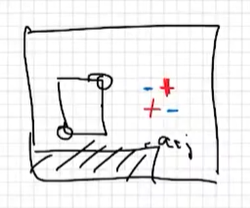
\includegraphics[width=0.4\textwidth]{images/70-75_2dd}
\end{wrapfigure}
Рассмотрим массив $B_{i,j}$ такой, что
$$b_{i,j} = a_{i,j}-a_{i-1,j}-a_{i,j-1}+a_{i-1,j-1}$$
\par Тогда при запросе 2 изменения будут только в двух вершинах прямоугольника (которые обведены в кружок)
Аналогично:
$$a_{i,j}=\sum_{u=0}^{i}\sum_{w=0}^{j}b_{u,w}$$
\newline Теперь посчитаем сумму на префиксе:
$$\sum_{x=0}^{i}\sum_{y=0}^{j}a_{x,y}=\sum_{x=0}^{i}\sum_{y=0}^{j}\sum_{u=0}^{x}\sum_{w=0}^{y}b_{u,w} = \sum_{u=0}^{i}\sum_{w=0}^{j}b_{u,w}\cdot (x-u+1)\cdot(y-w+1)$$
Обозначим два знака суммирования за один без индексов и тогда
$$xy\cdot \sum b_{u,w}+x\cdot \sum b_{u,w}\cdot(1-w)+y\cdot \sum b_{u,w}\cdot(1-u)+\sum b_{u,w}\cdot(1-w)\cdot(1-u)$$
Таким образом нам необходимо 4 дерева Фенвика.
\\ \par \textbf{Замечание: } Если $d$-мерная таблица, то $2^d$ деревьев Фенвика.
\setcounter{section}{74}
\section{Дерево Фенвика деревьев Фенвика: применение и асимптотика. }
\begin{wrapfigure}{L}{0.4\textwidth}
\vspace{-2ex}
\centering
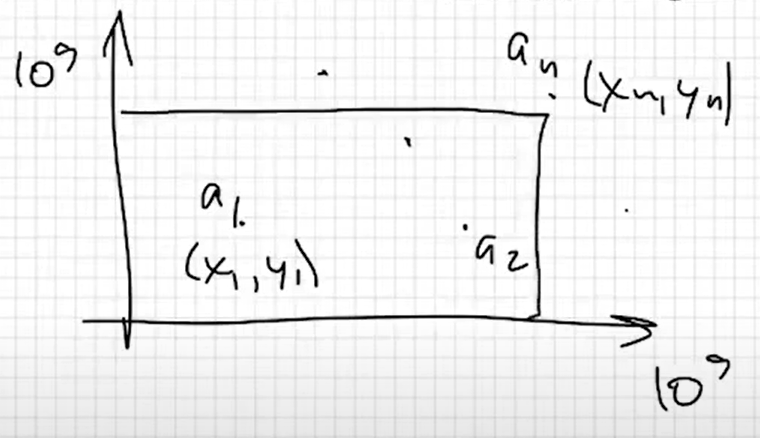
\includegraphics[width=0.4\textwidth]{images/70-75_ff2}
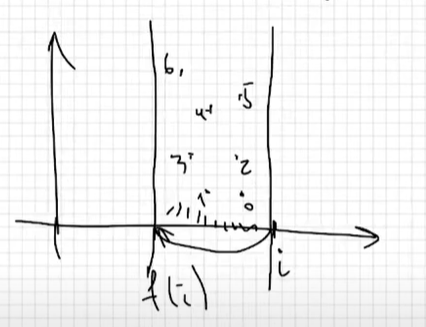
\includegraphics[width=0.4\textwidth]{images/70-75_ff1}
\end{wrapfigure}
Дана плоскость размера $10^9\times 10^9$, задается $n$ неизменяемых точек таких, что $n\leq 10^5$ и возможны запросы двух видов:
\begin{enumerate}
    \item $a_{(x,y)}= a_{(x,y)} + val$
    \item $\sum_{x_i,y_i}^{l,r}a_{x_i,y_i}$
\end{enumerate}
\textbf{1. Сжатие координат:} \quad  $x_i,y_i \leq n$
\\ \newline \textbf{2. Построение дерева Фенвика:}
\newline Для каждого $i$ создадим список точек $L_i$, у которых координата $x$ удовлетворяет условию $F(x)\leq x \leq i$. Отсортируем этот список по координате $y$ и построим на этом списке свое дерево Фенвика со своей индексацией.
\\ \par \noindent Тогда для ответа на 1 запрос мы обходим все маленькие деревья Фенвика, для которых выполнено условие $F(x)\leq x \leq i$. А в каждом маленьком дереве Фенвика бинпоиском по координате $y$ находим необходимую точку. \underline{Асимптотика:} $O(\log ^2 n)$
\\ \par \noindent А для ответа на 2 запрос (поиска префиксной суммы) мы также обходим все маленькие деревья Фенвика, для которых выполнено условие $F(x)\leq x \leq i$. А в каждом маленьком дереве Фенвика берем префисную сумму по координате $y$. \underline{Асимптотика:} $O(\log ^2 n)$
\\ \par \noindent \underline{Память:} $O(n\log n)$, так как каждая точка $(x,y)$ из $n$ штук хранится в логарифмическом количестве (маленьких) деревьев Фенвика.